%% Supplementary Material for the IEEE JBHI submission (single-blind).
%% Build: pdflatex supplement && bibtex supplement && pdflatex supplement && pdflatex supplement
%% Content source: the appendices of the earlier manuscript plus results/final/*.txt|*.md
%% (every number verified against those files; results/final supersedes the earlier manuscript).
\documentclass[9pt,journal]{IEEEtran}

\usepackage[T1]{fontenc}
\usepackage{amsmath,amssymb}
\usepackage{booktabs}
\usepackage{array}
\usepackage{graphicx}
\usepackage{url}
\usepackage{placeins}
\usepackage[hidelinks]{hyperref}
\hypersetup{pdfauthor={Sharoon Sharif},pdftitle={Supplementary Material for: One Checkpoint for Complete, Slide-Only and RNA-Only Patients: Auditing and Training Histology\textendash Transcriptomics Survival Models for Missing Inputs}}

\newcommand{\tabsize}{\scriptsize}
\newcommand{\pq}{PathQ-Former}
\newcommand{\pqf}{PQF}
\newcommand{\pqm}{PQF$^{-}$}
\newcommand{\cindex}{C-index}
\newcommand{\pmv}[2]{#1\,$\pm$\,#2}
\newcolumntype{R}[1]{>{\raggedright\arraybackslash}p{#1}}

\renewcommand{\thesection}{S-\Roman{section}}
\renewcommand{\thetable}{S\arabic{table}}
\renewcommand{\thefigure}{S\arabic{figure}}
\renewcommand{\theequation}{S\arabic{equation}}

% Float packing: many short tables, so allow several floats per page and small gaps.
\setcounter{topnumber}{6}
\setcounter{dbltopnumber}{6}
\setcounter{totalnumber}{10}
\renewcommand{\topfraction}{0.95}
\renewcommand{\dbltopfraction}{0.95}
\renewcommand{\textfraction}{0.05}
\renewcommand{\floatpagefraction}{0.85}
\renewcommand{\dblfloatpagefraction}{0.85}
\setlength{\floatsep}{6pt plus 1pt minus 1pt}
\setlength{\dblfloatsep}{6pt plus 1pt minus 1pt}
\setlength{\textfloatsep}{8pt plus 2pt minus 2pt}
\setlength{\dbltextfloatsep}{8pt plus 2pt minus 2pt}

\begin{document}

\title{Supplementary Material for: One Checkpoint for Complete, Slide-Only and RNA-Only Patients: Auditing and Training Histology--Transcriptomics Survival Models for Missing Inputs}

\author{Sharoon~Sharif%
\thanks{Manuscript received October XX, 2026.}%
\thanks{S. Sharif is with the Department of Electrical Engineering and Computer Science, Alabama A\&M University, Normal, AL 35762 USA, and with Faith Comes By Hearing, Albuquerque, NM USA (e-mail: ADD-EMAIL).}}

\markboth{Supplementary Material, submitted to the IEEE Journal of Biomedical and Health Informatics}%
{Sharif: Supplementary Material}

\maketitle

\section{Protocol and Methods}
\label{sec:protocol}
``S''-prefixed sections, tables, figures and equations are in this document; unprefixed ones are in the main paper. In the tables, \pqf{} denotes \pq{} and \pqm{} its variant without auxiliary heads. Table~\ref{tab:protocol} states the evaluation protocol, identical for every method, and Table~\ref{tab:methods} the methods and seeds. SurvPath (official implementation, published hyper-parameters, 4,096 patches per slide, 21.2\,M parameters), ABMIL, SNN and the two-layer RNA MLP use the hyper-parameters of the SurvPath repository; none was tuned under this protocol. \pq{} reads all patches of a patient (6,214 for the median of the 40 profiled BLCA fold-0 patients, Table~\ref{tab:efficiency}) and has 16.9\,M parameters including the pathway MLPs. Every results table (Section~\ref{sec:tables} here, Section~IV of the main paper) is regenerated from the archived per-run files by \texttt{scripts/reproduce\_tables.sh} in the code repository (\url{https://github.com/SharoonSharif/PathQFormer}; Zenodo DOI 10.5281/zenodo.22900123). Bracketed reference numbers refer to the reference list of the main paper.

\begin{table}[!t]
\caption{Evaluation protocol, identical for all methods.}
\label{tab:protocol}
\centering
\tabsize
\setlength{\tabcolsep}{3pt}
\begin{tabular}{@{}R{0.15\columnwidth}R{0.82\columnwidth}@{}}
\toprule
Aspect & Choice \\
\midrule
Unit & patient; all slides of a patient concatenated \\
Splits & SurvPath's five-fold patient-level splits; the validation fold is the reported fold \\
Endpoints & disease-specific survival (primary); overall survival (secondary) \\
Time bins & quartiles of uncensored training patients, outer edges $\pm\infty$, reused for validation \\
Metrics & Harrell's \cindex{} on continuous time [43], [44] (primary); Uno's IPCW \cindex{} [45] truncated at the 75th percentile of training event times, integrated Brier score [46] on the interior quartile grid, log-rank test at the median risk split (secondary) \\
Budget, seeds & 20 epochs, final checkpoint; seeds 0, 1, 2 with the fold index added \\
Statistics & one value per (cohort, fold) = mean over seeds; paired $t$ and exact Wilcoxon tests over the 25 pooled folds, 95\% percentile-bootstrap CI (10,000 resamples); per-cohort tests ($n = 5$) Holm-adjusted, exploratory \\
Audit & each input removed or permuted across patients; 10--50\% of patients missing one modality at random (five draws); Spearman correlation of fused and single-input risks \\
\bottomrule
\end{tabular}
\end{table}

\begin{table}[!t]
\caption{Methods and seeds under the 20-epoch DSS protocol. One BRCA run of each single-modality \pq{} is missing at seed 2.}
\label{tab:methods}
\centering
\tabsize
\setlength{\tabcolsep}{3pt}
\begin{tabular}{@{}llcl@{}}
\toprule
Method & Inputs & Seeds & Also run under \\
\midrule
SurvPath (official) & WSI+RNA & 3 & OS (1); 10 epochs (3) \\
ABMIL & WSI & 3 & -- \\
SNN & RNA & 3 & -- \\
RNA MLP (two layers) & RNA & 3 & -- \\
Slide-only \pq{} & WSI & 3 (BRCA 2) & -- \\
RNA-only \pq{} & RNA & 3 (BRCA 2) & -- \\
Late fusion & WSI+RNA & 2 & -- \\
\pqm{} & WSI+RNA & 3 & 10 epochs (3); Table~\ref{tab:ablate} (1) \\
\pqf{} & WSI+RNA & 3 & OS (1); Table~\ref{tab:finalconfig} (1) \\
\bottomrule
\end{tabular}
\end{table}

\section{Training Details and Selection History}
\label{sec:training}
\textit{Query blocks.} Each modality $m \in \{h, g\}$ has $K = 32$ learned queries $Q^m \in \mathbb{R}^{K \times d}$ with $d = 256$ and a stack of $L = 2$ pre-norm blocks,
\begin{align}
Q &\leftarrow Q + \mathrm{CA}\big(\mathrm{LN}(Q),\, U^m\big), \\
Q &\leftarrow Q + \mathrm{SA}\big(\mathrm{LN}(Q)\big),\qquad Q \leftarrow Q + \mathrm{FFN}\big(\mathrm{LN}(Q)\big),
\end{align}
where $U^m$ are the modality's input tokens (the LayerNormed patch embeddings, or the 275 pathway tokens produced by per-pathway two-layer MLPs of hidden width 128), $\mathrm{CA}$ is 8-head cross-attention with queries from $Q$ and keys and values from $U^m$, $\mathrm{SA}$ is self-attention among the queries and $\mathrm{FFN}$ a two-layer feed-forward network. Cross-attention over $N$ input tokens costs $O(KNd)$ and attention among the queries $O(K^2 d)$; the block returns 32 vectors, so the fusion stage does not depend on $N$. The fused codes pass through two Transformer encoder layers ($d = 256$, 8 heads) and a learned-query attention pooling; a linear layer with a sigmoid produces the $T = 4$ hazards (Table~\ref{tab:training}).

\begin{table}[!t]
\caption{Training configuration of \pq{} and of the official SurvPath baseline. Eq.~(1) is the discrete-time negative log-likelihood of the main paper.}
\label{tab:training}
\centering
\tabsize
\setlength{\tabcolsep}{3pt}
\begin{tabular}{@{}R{0.14\columnwidth}R{0.45\columnwidth}R{0.33\columnwidth}@{}}
\toprule
Setting & \pq{} & SurvPath (official) \\
\midrule
Epochs & 20, final checkpoint & 20, final checkpoint \\
Optimizer & AdamW [49], lr $10^{-4}$, wd $10^{-4}$, 1 warm-up epoch, cosine decay & RAdam [50], lr $5 \times 10^{-4}$ (published), wd $10^{-4}$ \\
Batch & 1 patient, gradient accumulation 2, gradient clip 1.0 & 1 patient \\
Dropout & 0.25; modality dropout 0.15 & 0.1 \\
Patches & all patches of all slides & 4,096-patch subsample (published) \\
Loss & Eq.~(1), censored term unweighted; auxiliary heads $\lambda = 0.5$ (full model) or 0 & Eq.~(1), censored term weighted 0.5 (published) \\
Sampling & uniform over training patients & weighted by (bin, censorship) (published) \\
Genes & min--max to $[-1, 1]$, fit on the training split & same \\
Parameters & 16.9\,M & 21.2\,M \\
\bottomrule
\end{tabular}
\end{table}

\textit{Selection history.} The base hyper-parameters of \pq{} (learning-rate schedule, dropout, modality-dropout rate, number of queries, fusion depth) were chosen on BLCA under the 10-epoch budget from the single-seed ablation runs in Table~\ref{tab:ablate}; none is distinguishable at one seed, and the chosen values are defaults rather than optima. The budget was raised from 10 to 20 epochs after inspecting the pooled validation curves of \pq{} and SurvPath under the 10-epoch budget; the 20-epoch curves (Fig.~\ref{fig:epochs}; the per-cohort curves, \path{epoch_curves_by_cohort.pdf}, are in the repository) show SurvPath flat from about epoch 7 and both \pq{} variants rising until about epoch 13--18. The learning rate and gradient-accumulation setting of \pq{} were changed at the same time as the budget, so the 10- and 20-epoch results are not a pure budget comparison; a single-seed check at lr $2 \times 10^{-4}$ on BLCA under the 20-epoch budget did not improve on the default (0.615 vs 0.630; its seed-averaged margin over SurvPath on the five BLCA folds was $+0.020$, 3 of 5 folds, against $+0.036$ for the default). The auxiliary-head variant and $\lambda = 0.5$ were adopted after the 20-epoch results of the variant without auxiliary heads on all five cohorts had been seen; the two variants are therefore reported as co-primary throughout, and no per-cohort result on BLCA is treated as confirmatory. Best-epoch validation scores were logged but used only in the selection replay (Table~\ref{tab:selection}).

\begin{figure}[!t]
\centering
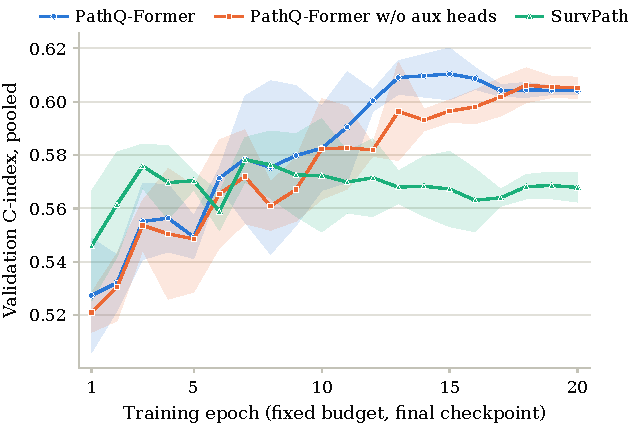
\includegraphics[width=\columnwidth]{figures/epoch_curves_pooled}
\caption{Validation \cindex{} per training epoch under the 20-epoch budget, pooled over all cohorts and folds, for \pq{}, its variant without auxiliary heads (`w/o aux heads') and SurvPath: mean over three seeds, $\pm$1 sd band over seeds. All results use the final epoch; the curves only set the budget.}
\label{fig:epochs}
\end{figure}

\section{Full Tables}
\label{sec:tables}
Table~\ref{tab:tests} completes the seed-averaged paired comparisons of Table~IV of the main paper with the unimodal baselines against SurvPath: none differs from SurvPath pooled (every CI spans zero). Table~\ref{tab:percohort} gives the per-cohort tests: on DSS, BRCA is the only cohort with a raw $p < 0.05$ and it does not survive Holm correction; on OS (one seed) BLCA, the development cohort, survives under the $t$-test only (Holm $p = 0.039$; Wilcoxon 0.312).

\begin{figure*}[!t]
\centering
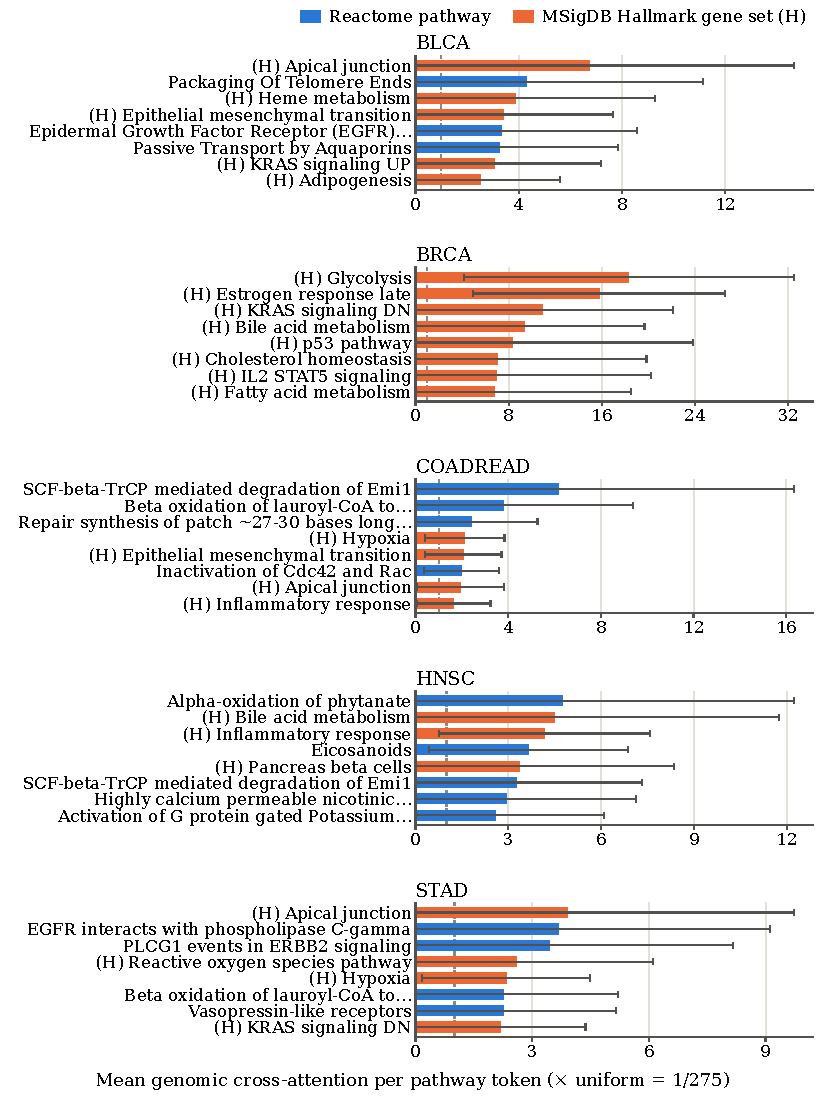
\includegraphics[angle=90,width=0.6\textwidth]{figures/pathway_importance_v2}
\caption{Pathway tokens with the highest mean genomic-query attention per cohort (\pq{}, 20 epochs, seed 0), as a multiple of uniform attention over the 275 tokens (dashed line), averaged over validation patients and the five folds (rotated). Blue: Reactome; orange, (H): MSigDB Hallmark. Error bars: mean $\pm$ sd over the five folds, clipped at zero; names over 45 characters are shortened.}
\label{fig:pathways}
\end{figure*}

\begin{figure*}[!t]
\centering
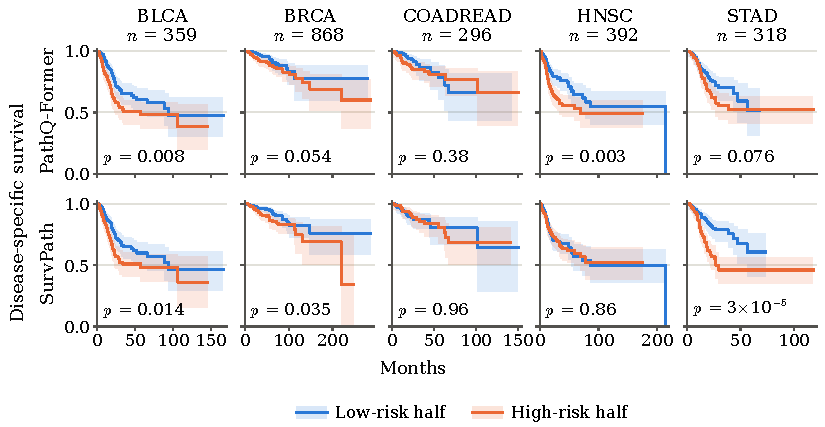
\includegraphics[width=0.68\textwidth]{figures/km_grid}
\caption{Kaplan--Meier curves of disease-specific survival for the high- and low-risk halves of the pooled out-of-fold validation predictions (20 epochs, seed 0); top: \pq{}, bottom: SurvPath. Patients are split at the median predicted risk of their own validation fold and the folds pooled, so every patient appears once. Bands: 95\% CI; $p$: log-rank test between the halves.}
\label{fig:km}
\end{figure*}

\begin{table}[!t]
\caption{Seed-averaged paired tests of the unimodal baselines against SurvPath over the 25 pooled (cohort, fold) units (DSS, 20 epochs, three seeds): mean $\Delta$ \cindex{}, 95\% bootstrap CI, $t$-test and Wilcoxon $p$, folds won. The eight remaining comparisons are Table~IV of the main paper.}
\label{tab:tests}
\centering
\tabsize
\setlength{\tabcolsep}{3pt}
\begin{tabular}{@{}lrlccc@{}}
\toprule
Comparison & $\Delta$ & 95\% CI & $t$ $p$ & W $p$ & Wins \\
\midrule
ABMIL vs SurvPath & $+0.001$ & $[-0.024, +0.026]$ & 0.95 & 0.85 & 14/25 \\
SNN vs SurvPath & $-0.007$ & $[-0.060, +0.045]$ & 0.80 & 0.73 & 10/25 \\
RNA MLP vs SurvPath & $+0.024$ & $[-0.027, +0.077]$ & 0.38 & 0.41 & 15/25 \\
\bottomrule
\end{tabular}
\end{table}

\begin{table}[!t]
\caption{Per-cohort seed-averaged paired differences against SurvPath (five folds per cohort): raw and Holm-adjusted $p$-values ($t$ and Wilcoxon adjusted separately), from unrounded values. $^\dagger$Development cohort.}
\label{tab:percohort}
\centering
\tabsize
\setlength{\tabcolsep}{3pt}
\begin{tabular}{@{}lrccc@{}}
\toprule
Cohort & $\Delta$ & $t$ $p$ (Holm) & W $p$ (Holm) & Wins \\
\midrule
\multicolumn{5}{@{}l}{\emph{\pqf{} vs SurvPath (DSS, three seeds)}} \\
BLCA$^\dagger$ & $+0.036$ & 0.175 (0.700) & 0.312 (1.000) & 3/5 \\
BRCA & $+0.086$ & 0.017 (0.084) & 0.062 (0.312) & 5/5 \\
COADREAD & $+0.044$ & 0.583 (1.000) & 0.625 (1.000) & 4/5 \\
HNSC & $+0.031$ & 0.544 (1.000) & 0.625 (1.000) & 4/5 \\
STAD & $-0.015$ & 0.719 (1.000) & 0.625 (1.000) & 2/5 \\
\multicolumn{5}{@{}l}{\emph{\pqm{} vs SurvPath (DSS, three seeds)}} \\
BLCA$^\dagger$ & $+0.015$ & 0.518 (1.000) & 0.625 (1.000) & 3/5 \\
BRCA & $+0.075$ & 0.073 (0.367) & 0.125 (0.625) & 4/5 \\
COADREAD & $+0.068$ & 0.202 (0.807) & 0.188 (0.750) & 4/5 \\
HNSC & $+0.023$ & 0.580 (1.000) & 0.625 (1.000) & 4/5 \\
STAD & $+0.006$ & 0.847 (1.000) & 0.812 (1.000) & 2/5 \\
\multicolumn{5}{@{}l}{\emph{\pqf{} vs SurvPath (OS, seed 0)}} \\
BLCA$^\dagger$ & $+0.043$ & 0.008 (0.039) & 0.062 (0.312) & 5/5 \\
BRCA & $+0.073$ & 0.015 (0.058) & 0.062 (0.312) & 5/5 \\
COADREAD & $-0.015$ & 0.578 (0.578) & 0.625 (0.625) & 2/5 \\
HNSC & $+0.025$ & 0.046 (0.138) & 0.125 (0.375) & 4/5 \\
STAD & $+0.044$ & 0.230 (0.460) & 0.312 (0.625) & 3/5 \\
\bottomrule
\end{tabular}
\end{table}

Table~\ref{tab:os} reports the overall-survival endpoint (one seed): \pq{} leads SurvPath by 0.034 pooled, and the same checkpoint keeps a \cindex{} of 0.531--0.586 with the RNA removed and 0.550--0.592 with the slide removed; with half of the validation patients missing one modality at random its OS \cindex{} changes by at most 0.021 (BRCA, 0.596 to 0.576; BLCA, COADREAD and HNSC by 0.005, STAD by 0.012). Table~\ref{tab:e10} reports the 10-epoch budget: the variant without auxiliary heads leads SurvPath by 0.028 pooled (18 of 25 folds), COADREAD being the only cohort with a raw $t$-test $p < 0.05$ (not a pure budget comparison; Section~\ref{sec:training}).

\begin{table}[!t]
\caption{Overall survival (20 epochs, seed 0): five-fold mean \cindex{} $\pm$ sd over folds, and the \pq{} checkpoint with one input removed (null codes). $^\dagger$Development cohort.}
\label{tab:os}
\centering
\tabsize
\setlength{\tabcolsep}{2.5pt}
\begin{tabular}{@{}lccrcc@{}}
\toprule
Cohort & \pqf{} & SurvPath & $\Delta$ & RNA rem. & Slide rem. \\
\midrule
BLCA$^\dagger$ & \pmv{0.595}{0.053} & \pmv{0.552}{0.056} & $+0.043$ & 0.576 & 0.592 \\
BRCA & \pmv{0.596}{0.043} & \pmv{0.523}{0.052} & $+0.073$ & 0.531 & 0.556 \\
COADREAD & \pmv{0.581}{0.132} & \pmv{0.596}{0.153} & $-0.015$ & 0.586 & 0.562 \\
HNSC & \pmv{0.536}{0.036} & \pmv{0.510}{0.029} & $+0.025$ & 0.535 & 0.550 \\
STAD & \pmv{0.603}{0.070} & \pmv{0.559}{0.045} & $+0.044$ & 0.574 & 0.582 \\
\midrule
Pooled & 0.582 & 0.548 & $+0.034$ & & \\
\bottomrule
\end{tabular}
\end{table}

\begin{table}[!t]
\caption{10-epoch budget (DSS, three seeds): \cindex{} mean $\pm$ sd over seeds of the five-fold mean, and the seed-averaged paired difference (pooled: 25 folds, 18 won). $^\dagger$Development cohort.}
\label{tab:e10}
\centering
\tabsize
\setlength{\tabcolsep}{3pt}
\begin{tabular}{@{}lccrcc@{}}
\toprule
Cohort & \pqm{} & SurvPath & $\Delta$ & $t$ $p$ & W $p$ \\
\midrule
BLCA$^\dagger$ & \pmv{0.618}{0.014} & \pmv{0.589}{0.004} & $+0.029$ & 0.272 & 0.312 \\
BRCA & \pmv{0.600}{0.031} & \pmv{0.536}{0.015} & $+0.064$ & 0.142 & 0.188 \\
COADREAD & \pmv{0.646}{0.046} & \pmv{0.551}{0.022} & $+0.094$ & 0.015 & 0.062 \\
HNSC & \pmv{0.556}{0.007} & \pmv{0.568}{0.035} & $-0.013$ & 0.595 & 1.000 \\
STAD & \pmv{0.574}{0.025} & \pmv{0.607}{0.012} & $-0.033$ & 0.471 & 0.625 \\
\midrule
Pooled & 0.599 & 0.570 & $+0.028$ & 0.079 & 0.063 \\
\bottomrule
\end{tabular}
\end{table}

Table~\ref{tab:secondary} reports the secondary metrics; the integrated Brier score (IBS, lower is better) is undefined on BRCA fold 4 for every method, so that fold is dropped from the paired units ($n = 24$). Uno's \cindex{} tracks Harrell's: \pq{} leads SurvPath by 0.039 and the variant without auxiliary heads by 0.046. Each of the four other methods beats SurvPath on the IBS by about 0.07 (Wilcoxon $p < 10^{-4}$): SurvPath's hazards are poorly calibrated under this protocol (its published loss weights the censored term by 0.5), so the IBS is not a fair accuracy comparison and is reported for completeness only.

\begin{table*}[!t]
\caption{Secondary metrics (20-epoch DSS protocol): mean $\pm$ sd over three seeds of the five-fold mean, and the seed-averaged paired difference from SurvPath over the pooled folds (95\% bootstrap CI; $t$-test / Wilcoxon $p$). *Four folds (undefined on BRCA fold 4).}
\label{tab:secondary}
\centering
\tabsize
\setlength{\tabcolsep}{3pt}
\begin{tabular}{@{}lccccc@{}}
\toprule
 & \pqf{} & \pqm{} & ABMIL & RNA MLP & SurvPath \\
\midrule
\multicolumn{6}{@{}l}{\emph{Uno's IPCW \cindex{}}} \\
BLCA & \pmv{0.630}{0.009} & \pmv{0.612}{0.019} & \pmv{0.560}{0.014} & \pmv{0.605}{0.013} & \pmv{0.597}{0.010} \\
BRCA & \pmv{0.636}{0.012} & \pmv{0.648}{0.038} & \pmv{0.599}{0.012} & \pmv{0.598}{0.012} & \pmv{0.525}{0.049} \\
COADREAD & \pmv{0.616}{0.032} & \pmv{0.644}{0.009} & \pmv{0.629}{0.015} & \pmv{0.646}{0.025} & \pmv{0.592}{0.020} \\
HNSC & \pmv{0.589}{0.034} & \pmv{0.587}{0.012} & \pmv{0.563}{0.031} & \pmv{0.563}{0.013} & \pmv{0.556}{0.027} \\
STAD & \pmv{0.586}{0.019} & \pmv{0.601}{0.014} & \pmv{0.562}{0.029} & \pmv{0.550}{0.010} & \pmv{0.591}{0.011} \\
$\Delta$ vs SurvPath ($n = 25$), 95\% CI & $+0.039$ $[-0.016, +0.086]$ & $+0.046$ $[+0.004, +0.087]$ & $+0.010$ $[-0.019, +0.042]$ & $+0.020$ $[-0.031, +0.070]$ & \\
\quad $t$ $p$ / W $p$ & 0.153 / 0.042 & 0.045 / 0.042 & 0.526 / 0.751 & 0.455 / 0.474 & \\
\midrule
\multicolumn{6}{@{}l}{\emph{Integrated Brier score}} \\
BLCA & \pmv{0.205}{0.008} & \pmv{0.210}{0.004} & \pmv{0.202}{0.007} & \pmv{0.191}{0.002} & \pmv{0.268}{0.031} \\
BRCA* & \pmv{0.073}{0.000} & \pmv{0.082}{0.004} & \pmv{0.077}{0.002} & \pmv{0.075}{0.002} & \pmv{0.131}{0.005} \\
COADREAD & \pmv{0.077}{0.006} & \pmv{0.081}{0.003} & \pmv{0.097}{0.001} & \pmv{0.082}{0.002} & \pmv{0.110}{0.009} \\
HNSC & \pmv{0.221}{0.019} & \pmv{0.215}{0.011} & \pmv{0.205}{0.010} & \pmv{0.200}{0.005} & \pmv{0.341}{0.087} \\
STAD & \pmv{0.201}{0.006} & \pmv{0.189}{0.009} & \pmv{0.208}{0.013} & \pmv{0.204}{0.001} & \pmv{0.276}{0.043} \\
$\Delta$ vs SurvPath ($n = 24$), 95\% CI & $-0.070$ $[-0.100, -0.044]$ & $-0.071$ $[-0.101, -0.043]$ & $-0.068$ $[-0.100, -0.039]$ & $-0.075$ $[-0.108, -0.044]$ & \\
\quad $t$ $p$ / W $p$ & $<$0.001 / $<$0.001 & $<$0.001 / $<$0.001 & $<$0.001 / $<$0.001 & $<$0.001 / $<$0.001 & \\
\bottomrule
\end{tabular}
\end{table*}

Table~\ref{tab:corr} gives the risk-score correlations behind Section~IV-A of the main paper: the fused risk of \pq{} follows its own RNA-removed risk ($\rho = 0.83$ pooled) far more closely than its slide-removed risk (0.45), and the two single-input risks are nearly uncorrelated (0.15); the standard deviation over the 15 pairs of a cell is 0.06--0.24 and is in the archive. Table~\ref{tab:impute} gives the per-cohort values behind Section~IV-D: mean imputation of a removed slide costs the variant without auxiliary heads 0.069 against 0.030 with the null code, and \pq{} 0.035 against 0.025 (null-code rows: Table~II of the main paper).

\begin{table}[!t]
\caption{Risk-score correlations of \pq{} (20 epochs): Spearman $\rho$, mean over the 15 (fold, seed) pairs per cohort, with its own single-input risks (top) and the other methods' risks on the same fold and seed (bottom); Pooled: mean over the 75 pairs.}
\label{tab:corr}
\centering
\tabsize
\setlength{\tabcolsep}{3pt}
\begin{tabular}{@{}lcccccc@{}}
\toprule
Fused risk of \pqf{} vs & BLCA & BRCA & COADREAD & HNSC & STAD & Pooled \\
\midrule
own slide-removed risk & 0.42 & 0.36 & 0.53 & 0.47 & 0.45 & 0.45 \\
own RNA-removed risk & 0.90 & 0.85 & 0.73 & 0.84 & 0.82 & 0.83 \\
\quad (slide-rem.\ vs RNA-rem.) & 0.22 & 0.09 & 0.16 & 0.15 & 0.13 & 0.15 \\
\midrule
\pqm{} & 0.79 & 0.62 & 0.66 & 0.71 & 0.69 & 0.69 \\
SurvPath & 0.63 & 0.38 & 0.38 & 0.45 & 0.48 & 0.46 \\
ABMIL & 0.46 & 0.51 & 0.38 & 0.44 & 0.48 & 0.46 \\
RNA MLP & 0.42 & 0.26 & 0.37 & 0.29 & 0.41 & 0.35 \\
SNN & 0.38 & 0.23 & 0.36 & 0.29 & 0.43 & 0.34 \\
\bottomrule
\end{tabular}
\end{table}

\begin{table*}[!t]
\caption{Mean imputation on the same \pq{} checkpoints (20 epochs): \cindex{} with one input replaced by the training-mean patch embedding or gene vector (mean $\pm$ sd over three seeds of the five-fold mean; one seed for \pqm{}), and the pooled difference from the complete-input score over the 25 seed-averaged folds.}
\label{tab:impute}
\centering
\tabsize
\setlength{\tabcolsep}{4pt}
\begin{tabular}{@{}lcccccrcc@{}}
\toprule
Condition & BLCA & BRCA & COADREAD & HNSC & STAD & $\Delta$ & $t$ $p$ & W $p$ \\
\midrule
\multicolumn{9}{@{}l}{\emph{\pqf{}, mean imputation (three seeds)}} \\
RNA removed & \pmv{0.597}{0.003} & \pmv{0.607}{0.035} & \pmv{0.602}{0.012} & \pmv{0.589}{0.014} & \pmv{0.581}{0.018} & $-0.009$ & 0.29 & 0.49 \\
Slide removed & \pmv{0.595}{0.027} & \pmv{0.591}{0.060} & \pmv{0.580}{0.016} & \pmv{0.558}{0.024} & \pmv{0.521}{0.037} & $-0.035$ & 0.040 & 0.045 \\
\multicolumn{9}{@{}l}{\emph{\pqm{}, mean imputation (one seed)}} \\
RNA removed & 0.627 & 0.545 & 0.631 & 0.580 & 0.594 & $-0.010$ & 0.50 & 0.83 \\
Slide removed & 0.524 & 0.499 & 0.600 & 0.535 & 0.524 & $-0.069$ & $3\times10^{-4}$ & $2.5\times10^{-4}$ \\
\bottomrule
\end{tabular}
\end{table*}

\begin{table*}[!t]
\caption{Checkpoint selection replayed on the stored validation histories. (A) Final: fixed-budget final checkpoint; Early: validation-loss early stopping, patience 5; Min.\ loss: lowest validation loss; Oracle: highest validation \cindex{} (pooled means over (fold, seed) runs); $\Delta$: Early minus Final over the 25 seed-averaged folds; Sel.\,/\,Best: mean selected epoch / mean epoch of highest validation \cindex{}. (B) The earlier validation-loss campaign: reported \cindex{}, \cindex{} at the best and the final epoch trained, mean selected epoch / epochs trained.}
\label{tab:selection}
\centering
\tabsize
\setlength{\tabcolsep}{3pt}
\begin{tabular}{@{}lcccccccccc@{}}
\toprule
\multicolumn{11}{@{}l}{\emph{(A) Replay on the stored histories}} \\
Method & Budget & Folds & Final & Early & Min.\ loss & Oracle & $\Delta$ & $t$ $p$ & W $p$ & Sel.\,/\,Best \\
\midrule
\pqf{} & 20 & 75 & 0.604 & 0.546 & 0.558 & 0.689 & $-0.059$ & 0.016 & $8\times10^{-4}$ & 2.2 / 10.0 \\
\pqm{} & 20 & 75 & 0.605 & 0.516 & 0.527 & 0.687 & $-0.090$ & $3\times10^{-7}$ & $1\times10^{-6}$ & 1.8 / 9.9 \\
Slide-only \pq{} & 20 & 70 & 0.588 & 0.523 & 0.529 & 0.688 & $-0.065$ & 0.006 & 0.005 & 1.8 / 9.3 \\
RNA-only \pq{} & 20 & 70 & 0.567 & 0.532 & 0.539 & 0.681 & $-0.034$ & 0.062 & 0.080 & 1.4 / 9.7 \\
SurvPath (official) & 20 & 75 & 0.568 & 0.568 & 0.559 & 0.679 & $+0.000$ & 0.99 & 0.98 & 1.6 / 6.9 \\
ABMIL & 20 & 75 & 0.569 & 0.568 & 0.568 & 0.668 & $-0.001$ & 0.95 & 0.61 & 1.4 / 6.2 \\
SNN & 20 & 75 & 0.561 & 0.523 & 0.522 & 0.669 & $-0.038$ & 0.054 & 0.052 & 1.4 / 7.3 \\
RNA MLP & 20 & 75 & 0.592 & 0.565 & 0.565 & 0.679 & $-0.027$ & 0.078 & 0.075 & 1.2 / 7.2 \\
\pqm{} & 10 & 75 & 0.599 & 0.524 & 0.538 & 0.658 & $-0.075$ & $8\times10^{-6}$ & $2.7\times10^{-5}$ & 1.8 / 6.3 \\
SurvPath (official) & 10 & 75 & 0.570 & 0.560 & 0.560 & 0.663 & $-0.010$ & 0.55 & 0.47 & 1.4 / 4.5 \\
\midrule
\multicolumn{11}{@{}l}{\emph{(B) The earlier validation-loss campaign (selection actually applied in training)}} \\
Method & Budget & Folds & Reported & & & Best epoch & Final epoch & & & Sel.\,/\,Trained \\
\midrule
SurvPath (official) & 20 & 35 & 0.562 & & & 0.642 & 0.549 & & & 1.3 / 6.4 \\
ABMIL & 20 & 25 & 0.535 & & & 0.639 & 0.568 & & & 1.5 / 6.5 \\
SNN & 20 & 25 & 0.514 & & & 0.642 & 0.561 & & & 1.3 / 6.4 \\
RNA MLP & 20 & 25 & 0.545 & & & 0.659 & 0.578 & & & 1.2 / 6.3 \\
Earlier fusion configuration & 20 & 35 & 0.577 & & & 0.641 & 0.569 & & & 4.7 / 9.8 \\
\bottomrule
\end{tabular}
\end{table*}

Table~\ref{tab:ablate} gives the fusion-block ablations on BLCA under the 10-epoch budget (Section~\ref{sec:training}); the settings move the fused \cindex{} within 0.595--0.638, inside the fold standard deviation of 0.07--0.13, and are not distinguishable at one seed. Table~\ref{tab:finalconfig} ablates the final configuration under the 20-epoch budget on BLCA (one seed each, trained on a laptop CPU) against the seed-0 GPU run of the main campaign (0.625 with both inputs; 0.630 $\pm$ 0.010 over three seeds). Capping \pq{} at the 4,096 training patches per slide that SurvPath uses gives 0.626, so on this cohort the margin over SurvPath is not explained by \pq{} reading more patches; two time bins give 0.628 and eight 0.609; the 281 Xena pathway groups [56] give 0.628 and the 50 Hallmark gene sets alone 0.600, 0.025 below the 275-token Reactome and Hallmark set. With half of the validation patients missing one modality at random every variant stays within 0.015 of its complete-input score (10--30\%: in the archive); for the two-bin variant the RNA- and slide-permuted evaluations give 0.619 and 0.571. All differences are within one fold standard deviation (0.057--0.082) and single-seed.

\begin{table}[!t]
\caption{Fusion-block ablations on BLCA, 10-epoch budget (\pqm{}, seed 0): five-fold mean \cindex{} $\pm$ sd over folds, and with one input removed (null codes).}
\label{tab:ablate}
\centering
\tabsize
\setlength{\tabcolsep}{3pt}
\begin{tabular}{@{}lccc@{}}
\toprule
Variant & Both inputs & RNA rem. & Slide rem. \\
\midrule
Base ($K{=}32$, depth 2, mod.\ dropout 0.15) & \pmv{0.609}{0.069} & 0.602 & 0.630 \\
Modality dropout 0 & \pmv{0.634}{0.075} & 0.609 & 0.598 \\
Modality dropout 0.3 & \pmv{0.616}{0.068} & 0.624 & 0.648 \\
Modality dropout 0.5 & \pmv{0.635}{0.108} & 0.587 & 0.626 \\
$K = 16$ queries & \pmv{0.638}{0.070} & 0.615 & 0.615 \\
$K = 64$ queries & \pmv{0.634}{0.127} & 0.619 & 0.624 \\
Fusion depth 1 & \pmv{0.598}{0.124} & 0.584 & 0.611 \\
Fusion depth 3 & \pmv{0.595}{0.088} & 0.585 & 0.610 \\
\bottomrule
\end{tabular}
\end{table}

\begin{table}[!t]
\caption{Final-configuration ablations on BLCA, 20-epoch budget (\pqf{}, seed 0, laptop CPU): five-fold mean \cindex{} $\pm$ sd, with one input removed (null codes) and with 50\% of validation patients missing one modality at random (five draws per fold). Base: seed-0 GPU run (4 bins, 275 tokens, all patches).}
\label{tab:finalconfig}
\centering
\tabsize
\setlength{\tabcolsep}{3pt}
\begin{tabular}{@{}lcccc@{}}
\toprule
Variant & Both inputs & RNA rem. & Slide rem. & 50\% missing \\
\midrule
Base (seed 0, GPU) & \pmv{0.625}{0.081} & 0.598 & 0.588 & 0.618 \\
Time bins $T = 2$ & \pmv{0.628}{0.057} & 0.634 & 0.575 & 0.616 \\
Time bins $T = 8$ & \pmv{0.609}{0.082} & 0.578 & 0.605 & 0.604 \\
Hallmark only (50 tokens) & \pmv{0.600}{0.075} & 0.608 & 0.554 & 0.597 \\
Xena groups (281 tokens) & \pmv{0.628}{0.063} & 0.604 & 0.634 & 0.615 \\
4,096 patches per slide & \pmv{0.626}{0.059} & 0.591 & 0.622 & 0.611 \\
\bottomrule
\end{tabular}
\end{table}

Table~\ref{tab:selection} is the checkpoint-selection replay summarised in Section~IV-E of the main paper. Block (A) replays three post-hoc rules on the stored 20-epoch histories (three seeds; the single-modality \pq{}s have 70 instead of 75 fold histories): validation-loss early stopping (patience 5) costs the six \pq{}, SNN and MLP runs 0.027--0.090 pooled and ABMIL and SurvPath nothing, because the latter reach their best validation \cindex{} at epoch 6.2 and 6.9 against 7.2--10.0 for the others; the oracle rule, an unattainable bound biased in favour of every method, puts every method at 0.67--0.69. The two 10-epoch methods behave the same way (early stopping costs \pqm{} 0.075 and SurvPath 0.010). Block (B) is the earlier campaign that actually trained with validation-loss selection (patience 5, minimum 6 epochs, 20-epoch budget; 29 cohort-level runs, 145 folds; Section~\ref{sec:runs}): its reported \cindex{} is 0.063--0.128 below the best epoch of the same runs for every method. Selection and scoring use the same fold throughout, so every replayed rule is biased in its own favour and the oracle is an upper bound. (For the single-modality \pq{}s the run-weighted Final differs by 0.001--0.002 from the Pooled column of Table~III of the main paper, which averages the cohort means.)

\section{Efficiency}
\label{sec:efficiency}
Table~\ref{tab:efficiency} reports parameters, latency and peak GPU memory per patient (first 40 patients of the BLCA fold-0 validation set; medians on one RTX PRO 4000). At 4,096--6,214 patches the two models have equal forward latency; \pq{}'s training step takes 104\,ms against 176\,ms for SurvPath, and its peak memory on full slides is 1.17\,GiB against 1.74\,GiB. The claim is limited to these slide sizes on this GPU; neither implementation was profiled, and training throughput in practice was bound by reading features from storage.

\begin{table}[!t]
\caption{Compute per patient (BLCA fold-0 validation, first 40 patients, medians, one RTX PRO 4000): parameters (M), patches (6,214 = median patient), forward and forward+backward time (ms), peak GPU memory (GiB).}
\label{tab:efficiency}
\centering
\tabsize
\setlength{\tabcolsep}{3pt}
\begin{tabular}{@{}lrrrrr@{}}
\toprule
Model & Params & Patches & Fwd & Fwd+bwd & Mem. \\
\midrule
\pqf{} (all patches) & 16.9 & 6,214 & 35.0 & 104.2 & 1.17 \\
\pqf{} (4,096 patches) & 16.9 & 4,096 & 34.7 & 104.1 & 0.17 \\
SurvPath (as trained) & 21.2 & 4,096 & 35.7 & 175.6 & 0.20 \\
SurvPath (all patches) & 21.2 & 6,214 & 36.0 & 176.0 & 1.74 \\
\bottomrule
\end{tabular}
\end{table}

\section{Pathway Attention}
\label{sec:pathways}
The genomic query block exposes cross-attention from each query over the 275 pathway tokens. Fig.~\ref{fig:pathways} shows, per cohort, the eight tokens with the highest mean attention relative to uniform ($1/275$), averaged over validation patients and the five folds (seed 0). The top entries are 3.9 to 18.3 times the uniform weight, but the standard deviation over folds exceeds the mean for most of them (BLCA: apical junction, $6.7 \pm 7.9$; BRCA: glycolysis, $18.3 \pm 14.1$), so the ranking is descriptive only; attention weights are not a measure of feature importance [51].

\section{Kaplan--Meier Curves}
\label{sec:km}
Fig.~\ref{fig:km} shows disease-specific survival of the high- and low-risk halves of the pooled out-of-fold predictions (20 epochs, seed 0). The log-rank $p$-values between the halves are, for \pq{}, 0.008 (BLCA), 0.054 (BRCA), 0.38 (COADREAD), 0.003 (HNSC) and 0.076 (STAD), and for SurvPath 0.014, 0.035, 0.96, 0.86 and $3 \times 10^{-5}$. The pooled curves combine five fold models at one seed and are descriptive.

\section{Evaluation Pitfalls in Survival MIL Pipelines}
\label{sec:pitfalls}
Each of the following choices produces plausible-looking \cindex{} values in a survival MIL pipeline; ours avoids them as stated. (1)~\emph{Concordance on discrete bins} ties many pairs; Harrell's \cindex{} is computed on continuous time. (2)~\emph{Bin edges fit on the validation fold} put its labels on a different scale and leak its label distribution; edges are fit on uncensored training patients and reused. (3)~\emph{Slide-level samples} weight multi-slide patients several times; one sample per patient, all slides concatenated. (4)~\emph{Unscaled gene inputs} feed log-expression on an arbitrary scale to the pathway MLPs; genes are min--max scaled with training-split statistics. (5)~\emph{Selection on the reported fold} biases every rule upward (Table~\ref{tab:selection}); a fixed budget, the final checkpoint and several seeds avoid it. (6)~\emph{Non-standard risk and dropout semantics}, $1 - S(T)$ as the risk or modality dropout per batch; risk is $-\sum_t S(t)$ and dropout is per sample. (7)~\emph{Extreme times in the Brier grid} evaluate where a single patient is at risk; the interior quartile edges are used. (8)~\emph{Untruncated IPCW weights} diverge as the censoring survival function approaches zero; Uno's \cindex{} is truncated at the 75th percentile of training event times.

\section{Run Inventory and Compute}
\label{sec:runs}
The archive holds 204 cohort-level GPU runs, each of five folds, and 13 cohort-level runs trained on a laptop CPU. The GPU runs are: 34 in the first multi-cohort campaign, namely 24 under the earlier validation-loss protocol and the single-seed 10-epoch runs of \pq{} and SurvPath on five cohorts; 31 BLCA fusion-block ablations, late fusion and 10-epoch seeds 1--2 of \pq{} and SurvPath; 128 under the 20-epoch DSS protocol (the nine methods of Table~\ref{tab:methods} on five cohorts with the seeds listed there); 10 under the OS endpoint (\pq{} and SurvPath on five cohorts); and one 20-epoch learning-rate check on BLCA (Section~\ref{sec:training}). The laptop runs are the eight BLCA seed-0 runs of the validation-loss campaign and the five final-configuration ablations of Table~\ref{tab:finalconfig}. The validation-loss campaign (patience 5, minimum 6 epochs, 20-epoch budget) comprises 29 cohort-level runs with 145 folds: SurvPath, ABMIL, SNN, the RNA MLP and the earlier fusion configuration on five cohorts, with three seeds on BLCA for SurvPath and the fusion configuration (Table~\ref{tab:selection}B; three further BLCA \pq{} runs, one without warm-up and the slide-only and RNA-only variants of the earlier fusion configuration, are archived but not tabulated). It selected epoch 1 on median (mean 2.2; 82\% of folds epoch 1--3), trained 7.2 epochs on average, and reported a mean \cindex{} of 0.543 against 0.644 at the best epoch of the same runs, with 14 of 25 method $\times$ cohort cells within 0.45--0.55; at or below 0.55 the counts are STAD 4 of 5, HNSC 5 of 5 and BRCA 4 of 5, the exceptions being SurvPath on STAD (0.610) and SNN on BRCA (0.572). Replaying each run's own rule on its stored history reproduces the stored selected epoch and reported \cindex{} in 145 of 145 folds.

Across the 128 runs of the 20-epoch DSS protocol, the standard deviation of the \cindex{} over the five folds of a run ranges from 0.03 (SNN on BRCA at seed 1; both \pq{} variants on HNSC at seed 0) to 0.25 (COADREAD, \pq{} at seed 1); on COADREAD it is 0.12--0.25 for the fusion models and 0.05--0.25 over all methods, which is why per-cohort tests with five folds are exploratory. Every run stores its results, configuration, per-fold predictions and per-epoch histories (late-fusion runs: results and predictions only); GPU runs used rented RTX PRO 4000/4500 and RTX 2000 Ada GPUs sharing a network volume.

\end{document}
